%%%%%%%%%%%%%%%%%%%%%%%%%%%%%%%%%%%%%%%%%%%%%%%%%%%%%%%%%%%%%%%%%%%%%
%% This is a (brief) model paper using the achemso class
%% The document class accepts keyval options, which should include
%% the target journal and optionally the manuscript type.
%%%%%%%%%%%%%%%%%%%%%%%%%%%%%%%%%%%%%%%%%%%%%%%%%%%%%%%%%%%%%%%%%%%%%
\documentclass[journal=jacsat,manuscript=article]{achemso}

%%%%%%%%%%%%%%%%%%%%%%%%%%%%%%%%%%%%%%%%%%%%%%%%%%%%%%%%%%%%%%%%%%%%%
%% Place any additional packages needed here.  Only include packages
%% which are essential, to avoid problems later.
%%%%%%%%%%%%%%%%%%%%%%%%%%%%%%%%%%%%%%%%%%%%%%%%%%%%%%%%%%%%%%%%%%%%%
\usepackage{chemformula} % Formula subscripts using \ch{}
\usepackage[T1]{fontenc} % Use modern font encodings
\usepackage{graphicx}
\usepackage{enumerate}
\usepackage{enumitem}
\usepackage{indentfirst}
\setlength{\parindent}{2em}
\usepackage{siunitx}
\usepackage{hyperref}
%%\usepackage{url}


%%%%%%%%%%%%%%%%%%%%%%%%%%%%%%%%%%%%%%%%%%%%%%%%%%%%%%%%%%%%%%%%%%%%%
%% If issues arise when submitting your manuscript, you may want to
%% un-comment the next line.  This provides information on the
%% version of every file you have used.
%%%%%%%%%%%%%%%%%%%%%%%%%%%%%%%%%%%%%%%%%%%%%%%%%%%%%%%%%%%%%%%%%%%%%
%%\listfiles

\author{Zhenzhe Zhang}
\email{zhenzhe.zhang@mail.mcgill.ca}
%%\phone{+123 (0)123 4445556}
%%\fax{+123 (0)123 4445557}
\affiliation[McGill University]
{Department of Chemistry, McGill University, Montreal}

%%%%%%%%%%%%%%%%%%%%%%%%%%%%%%%%%%%%%%%%%%%%%%%%%%%%%%%%%%%%%%%%%%%%%
%% The document title should be given as usual. Some journals require
%% a running title from the author: this should be supplied as an
%% optional argument to \title.
%%%%%%%%%%%%%%%%%%%%%%%%%%%%%%%%%%%%%%%%%%%%%%%%%%%%%%%%%%%%%%%%%%%%%
\title{Adatoms in the surface Ullmann coupling}

\begin{document}

%%%%%%%%%%%%%%%%%%%%%%%%%%%%%%
%% The "tocentry" environment can be used to create an entry for the
%% graphical table of contents. It is given here as some journals
%% require that it is printed as part of the abstract page. It will
%% be automatically moved as appropriate.
%%%%%%%%%%%%%%%%%%%%%%%%%%%%%%%%%%%%%%%%%%%%%%%%%%%%%%%%%%%%%%%%%%%%%
\begin{tocentry}

Some journals require a graphical entry for the Table of Contents.
This should be laid out ``print ready'' so that the sizing of the
text is correct.

Inside the \texttt{tocentry} environment, the font used is Helvetica
8\,pt, as required by \emph{Journal of the American Chemical
Society}.

The surrounding frame is 9\,cm by 3.5\,cm, which is the maximum
permitted for  \emph{Journal of the American Chemical Society}
graphical table of content entries. The box will not resize if the
content is too big: instead it will overflow the edge of the box.

This box and the associated title will always be printed on a
separate page at the end of the document.

\end{tocentry}


\begin{abstract}
This manuscript reviews the results of experimental and computational studies of the surface Ullmann coupling that shed light on the role of surface adatoms in its mechanism. A particular focus is on the early stages of the polymerization and the coupling of just two monomers.
\end{abstract}

\newpage


\section{Introduction}


\subsection{``Classical'' Ullmann Coupling}

Ullmann reaction, named after Fritz Ullmann who discovered it in 1901, is a coupling reaction between two aryl halides in the presence of Cu-containing catalysts, in the creation of a C--C bond between the aromatic rings.  (Figure~\ref{fig:classical}). 
%
\begin{figure}[ht]
\centering
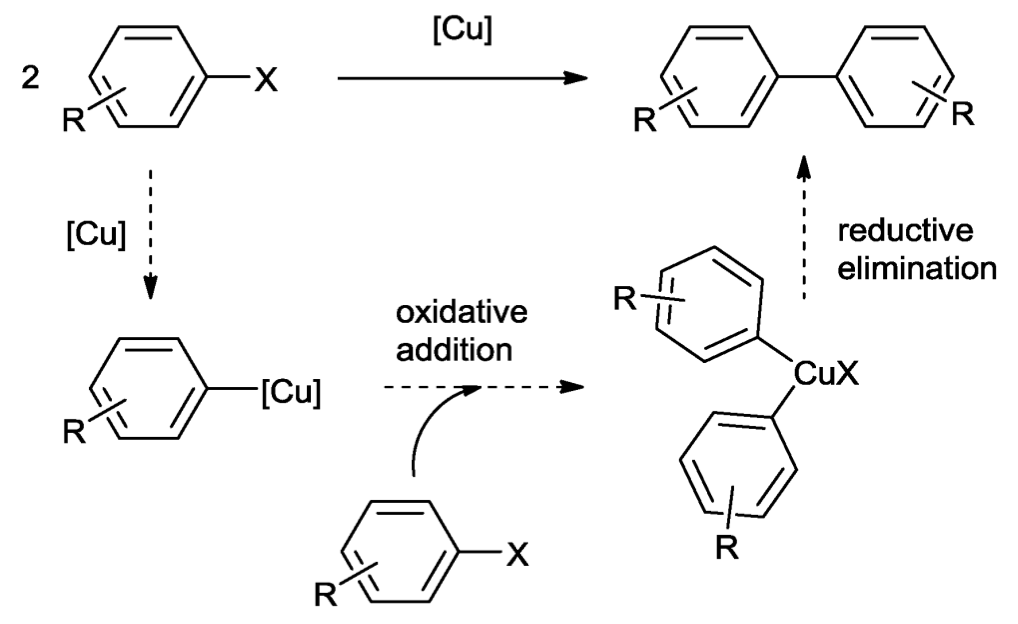
\includegraphics[scale=0.6]{Fig/Figure1-mechanism.png}
\caption{Mechanism of classic Ullmann coupling}
\label{fig:classical}
\end{figure}
%
% RZK: Reduce the "history" of the reaction to the first sentence, which mentions Ullmann. The second sentence should start discussing the utility of UC in modern chemistry.
Despite a variety of limitations ranging from harsh reaction conditions~\cite{RZK} and erratic yields~\cite{RZK} to ZZZ(RZK: any other problems?), the Ullmann coupling has become and still remains one of the key reactions to build C-C bonds in organic synthesis. 
% RZK: discuss very briefly the scope of reaction. What organic molecules can be coupled (...)? What leaving groups are used? Are they only halides? What metals/alloys are used? (always copper?)
Among the halides, iodine is the best leaving group but the use of bromine and chlorine has been widely reported~\cite{RZK}. 
In addition to halides, Ullmann coupling can occur with ZZZ as leaving groups~\cite{RZK}. 
In addition to the traditional aryl halides, synthesis of numerous (aromatic molecules?) {products} have been achieved via Ullmann coupling including N-aryl amines, ethers, aryl amides and amines. %RZK: the scope of organic substrates for Ullmann is probably much larger today. Extend the list and add citations.
%RZK: What metals (and/or their ions) are used in Ullmann coupling?

%organic molecules + leaving groups + catalysis
It is widely accepted that the Ullmann coupling proceeds via the formation of an organometallic intermediate (Figure~\ref{fig:classical}). 
This intermediate then reacts with another precursor with the formation of a ZZZ and a subsequent reductive elimination to form biaryl moieties (Figure.\ref{fig:classical}). 
%RZK: It is unclear from the figure how CuX returns to its active catalytic form.

%RZK: the next paragraph will be corrected AFTER ZHZH makes corrections above
Cu-catalyzed coupling has acquired great significance in the last decade due to its advantages such as (1) Cu is a cheaper alternative to palladium, platinum or rhodium; (2) avoidance of the halogen side-product; and (3) air or oxygen can act as oxidant. However, drawbacks still exit for large-scale development: (1) harsh conditions are necessary like high temperature and polar solvents with high boiling point; (2) poor solubility of many Cu compounds in solvent; (3) poor functional group tolerance.

Recent advances in the traditional Ullmann coupling reaction in solution have been reviewed by ZZZ. %RZK: cite recent reviews that discuss Ullmann in solution.


\subsection{Surface Ullmann Coupling}

A recent surge of interest in electronic devices based on low-dimensional organic nanostructures with $\pi$-conjugated backbones has led to a renewed attention to the Ullmann coupling reaction. 
In the case of low-dimensional materials, the well-established ability of the Ullmann coupling to create bonds between aromatic carbon atoms and couple their $\pi$ systems have been transferred from solution to metal surfaces, which serve as both a low-dimensional confining template and catalyst. 
The on-surface Ullmann reaction is currently viewed as a promising bottom-up strategy to assemble, in mild conditions, one- and two-dimensional organic polymers with high degree of control of their electronic properties~\cite{RZK-reviews}.

% RZK. How do we know this is the first study? [use "One of the first studies"] The focus of the study is not on synthesis but rather characterization of the mechanism. They say, phenyl is parallel to the surface. Was it confirmed later?
[RZK: One of] The first fundamental study[ies] of the [RZK: mechanism of the?] surface-confined coupling of iodobenzene to biphenyl under ultrahigh vacuum (UHV) condition was reported by Xi \textit{et al.} in 1992~\cite{sur_sci01}.
%
The intermediate species of the same reaction was inspected using STM imaging by Weiss and coworkers in 1998~\cite{langm01}.
%%ZHZH Dima asked what happened between 1992 and 2004? 
% RZK: Are there any papers on surface Ullmann coupling in this period? If yes, list them here. 
%
%RZK: discuss the conclusion with ZHZH.
%RZK: is there another, more modern and widely-accepted term to use instead of protopolymer?
In 2004, it was demonstrated that linear protopolymers -- aligned monomer units of a polymer that have not yet reacted to the final polymer -- can be obtained by depositing \textit{para}-diiodobenzene on Cu(111) at 77 K~\cite{jacs01}. 
%
%RZK: It is a strong statement to say that the field became popular after one publication. Is this publication really the first of its kind? How do you know that it was this publication that made the field well known?
%RZK: "covalently-bonded molecular nanostructures" does not sound right.
Remarkably, the first synthesis of covalently-bonded molecular nanostructures on metal surfaces under vacuum has employed the Ullmann reaction. The coupling between brominated tetraphenyl-porphyrins on the Au(111) surface (Figure~\ref{fig:first_model}) was performed by Grill and coworkers in 2007~\cite{Naturenano2007}. 

\begin{figure}[ht]
\centering
%RZK: do not use scale, use width like I show below
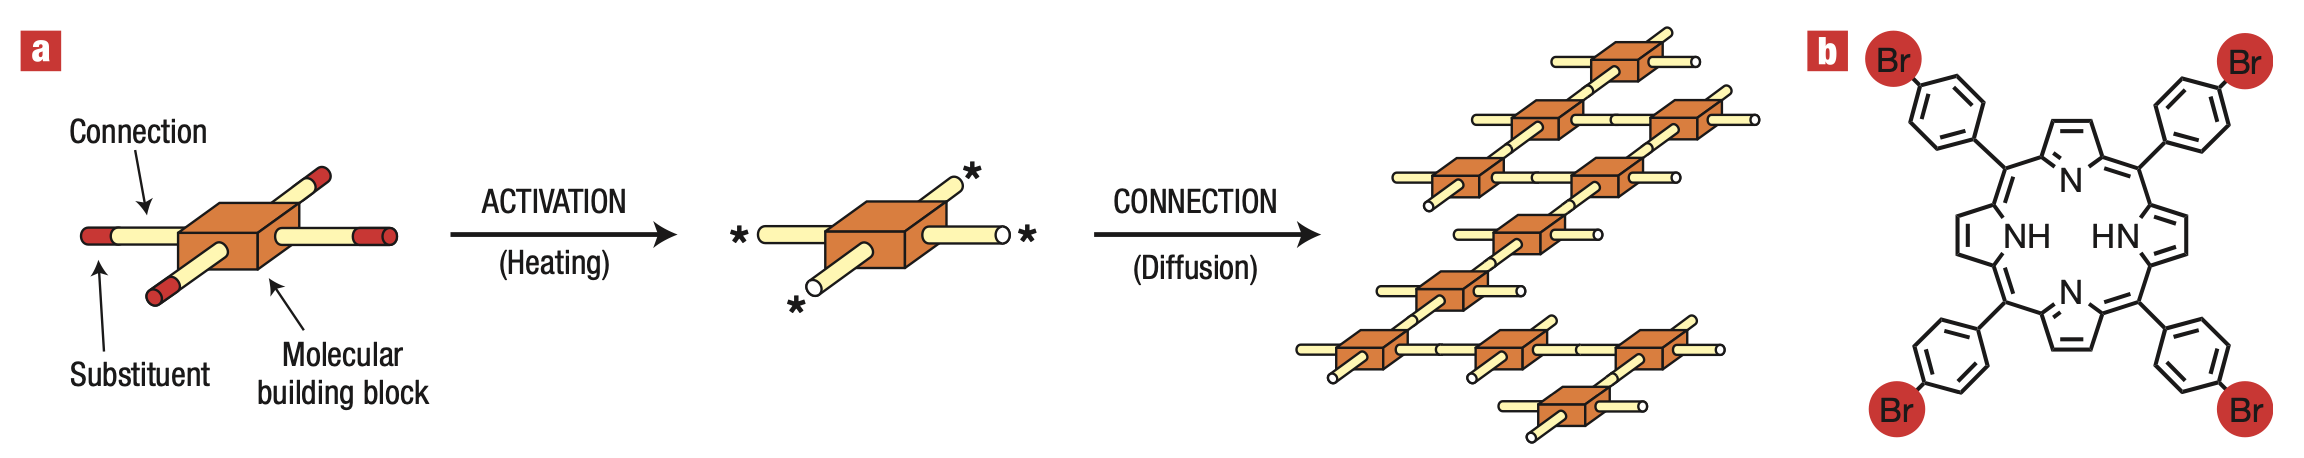
\includegraphics[width=0.95\textwidth]{Fig/Figure-2.png}
\caption{Macromolecular strucutrues formation from brominated tetraphenyl-porphyrins. Reprinted from~\cite{RZK} with permission of American Chemical Society or PUBLISHER.}
%RZK: If you take a figure from a publication it is very important to cite the work and obtain publisher's permission. We need to make sure that all our borrowed figures satisfy copyright permissions. For example, see: https://www.stm-assoc.org/2016_01_05_Guidelines_for_Quotation_From_Journal_Articles.pdf
\label{fig:first_model}
\end{figure}

Since then, surface Ullmann coupling has become one of the most representative on-surface synthesis scheme and has been utilized to create a variety of covalently-linked extended aromatic systems from halogenated aryl precursors on multiple metal surfaces~\cite{RZK-reviews}.


\subsection{Mechanism of Surface Ullmann Coupling}

Although multiple covalently-bonded nanostructures have been obtained on metal surfaces via Ullmann coupling, our knowledge of the mechanism of the surface processes still remains fragmentary. 
%
A thorough understanding of the mechanism of surface Ullmann coupling reaction will enable rational, faster, more precise design of the halogenated precursors, well-matched to a chosen metal surface.
%
%RZK: the following sentece does not belong here.
%The organometallic intermediates have been proven in existence in the mechanism investigation. %
%RZK: note how I refer to figures. Do not abbreviate "Fig.", use non-breaking space ~.
The overall coupling process can be divided into elementary steps depicted in Figure~\ref{fig_mecha}.

\begin{figure}[ht]
\centering
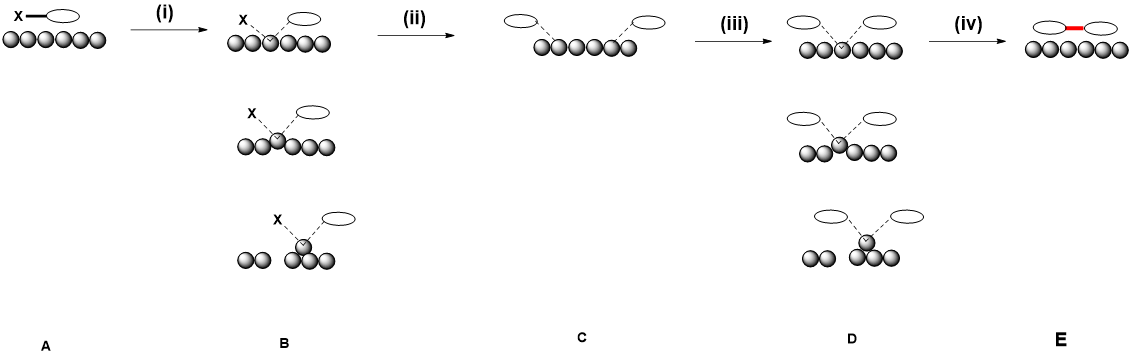
\includegraphics[width=0.95\textwidth]{achemso/Fig/mechanism.png}
%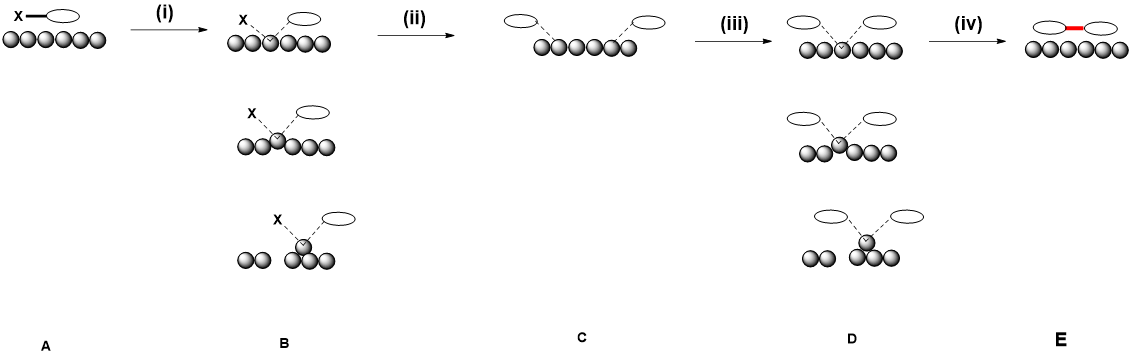
\includegraphics[scale=0.45]{achemso/Fig/mechanism.png}
\caption{Five steps in surface Ullmann coupling}
\label{fig_mecha}
\end{figure}

%%\begin{enumerate}[align=left, itemindent=2em, label=(\roman*)]
    %%\item Dehalogenation of Precursors [The fundamental step is the %%disassociate of halogens, the cleavage of C-X bonds (X = halogens) is %%usually activated by thermal, electron-induced and photon-simulated. %%The energy will vary from 0.05 ~ 0.80 eV with different X on different %%coinage surfaces.]
    %%\item Diffusion of single Dehalogenlated 'Radicals' [The removal of %%halogens from precursors results in unsaturated carbons (radicals), %%which interact with metal atoms to form C-Metal radical (C = %%dehalogenated precursor and Metal = Au, Ag or Cu). C-Metal radical %%will diffuse on metal surface and the metal atom interacting with the %%radical will shift.]
    %%\item The Formation of Organometallic Intermediates C-Metal-C from Two %%Single Radicals [Diffusion brings two single radical close to each %%other, and then these two species would form a dimerized %%organometallic intermediate before the appearance of coupling product]
    %%\item The Formation of Carbon-Carbon Bond []
    %%\item Diffusion of Coupling Product []
%%\end{enumerate}  


\subsubsection{Dehalogenation}

The fundamental step of surface Ullmann coupling is a dissociative dehalogenation of organic precursors. Upon adsorption, the carbon-halogen bond is broken with the aid of the catalytic properties of metal surface. In 2013, \citeauthor{jacs2013}\cite{jacs2013} proposed an activation barrier of 0.4-1.0 eV for exothermic dehalogenation by DFT simulations. In specific, bromobenzene and iodobenzene on Au(111), Ag(111) and Cu(111) surface displayed different reactivity, i.e., the activation barrier and reaction energy both decrease in the order Au > Ag > Cu, and for all surfaces studied, iodine substituents are 0.1-0.5 eV lower than bromine ones in dehalogenation [Fgiure.\ref{fig:dehalo}]. The trend is plausible due to the Bond-dissociation energy(BDE) of C-I is ~0.65 eV lower than C-Br\cite{Arpc1982}.

\begin{figure}[ht]
\centering
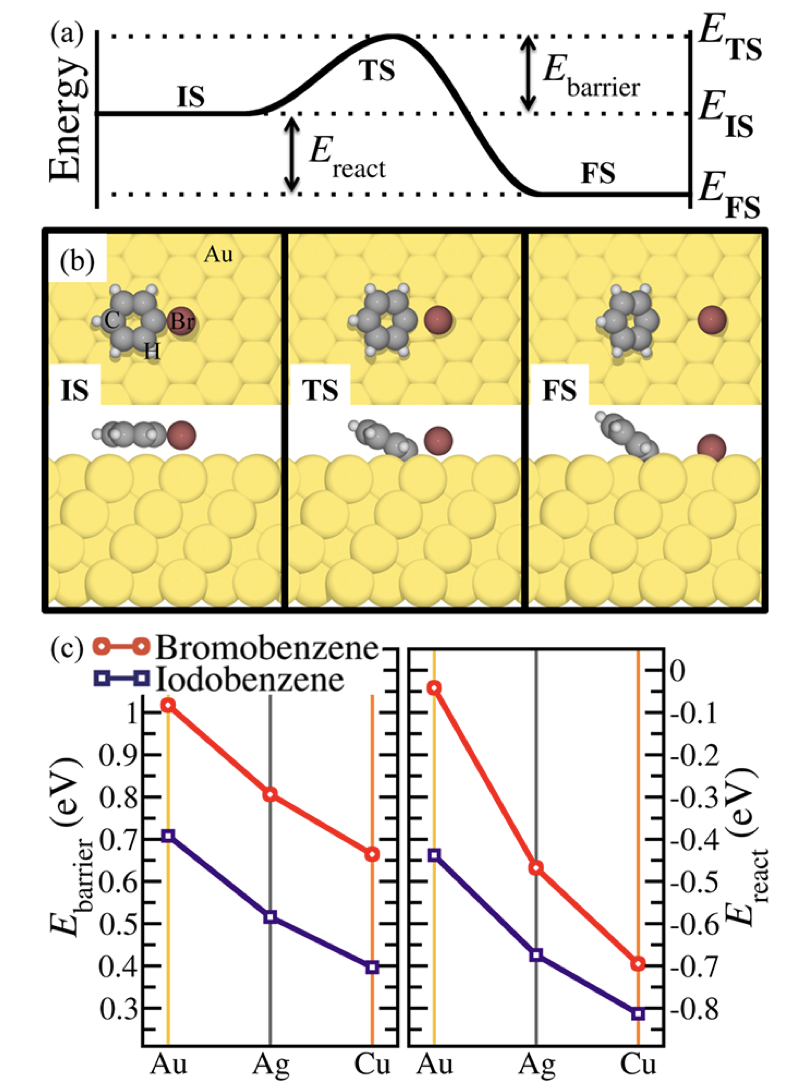
\includegraphics[scale=0.45]{achemso/Fig/dehalogentaion.png}
\caption{Dehalogenation Energy}
\label{fig:dehalo}
\end{figure}
This data also indicates the distinct influence of surfaces, which has been proven in experiment of bromobenzene and iodobenzene. For instance, the dissociaton of iodobenzene occurs at 175 K on Cu(111)\cite{sur_sci01}, ~200 K on Ag(111)\cite{sur_sci02} and ~250 K on Au (111)\cite{sur_sci03}. Same trend was demonstrated by bromobenzene with a higher temperature on all surfaces.


\subsubsection{Diffustion of Single "Radical"}
Dehalogenation results in unsaturated carbons (surface-stabled single radicals), where the dangling bonds of the unsaturated carbons bind to the adjacent metal atom. The diffusion accessibility of single radicals play a decisive role in further coupling process. Firstly, \citeauthor{langm01}\cite{langm01} observed the dehalogenated phenyl radical diffuses on Cu(111) at 77 K by STM. In 2010 \citeauthor{pccp2010}\cite{pccp2010} demonstrated theoretically that phenyl radical keeps a tilt angle of ~$36^\circ$ with respect to the Cu surface after dehalogenation. During the diffusion process, the phenyl radical overturns to become bound to a nearby atom on the surface [Figure.\ref{fig:4}]. The energy barrier of diffusion is estimated to ~0.09 eV for phenyl radical, which is consistent with the experimental temperature. However, the diffusion energy barrier and the tilt angle between single radical and substrate will change with the size increasing of reactant molecules.

\begin{figure}[ht]
\centering
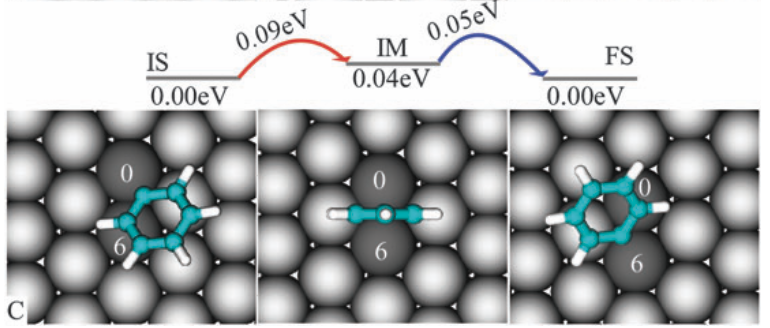
\includegraphics[scale=0.6]{achemso/Fig/overturn.png}
\caption{overturn}
\label{fig:4}
\end{figure}


\subsubsection{Formation of Dimerized Organometallic Intermediates}
A dimerized organometallic intermediate based on carbon-metal-carbon interlinks forms when two single radical diffuse close to each other. These carbon-metal-carbon bridges have been revealed in many cases. In 2011, \citeauthor{jacs2011}\cite{jacs2011} studied the organometallic intermediate of surface Ullmann coupling from dibromoterphenyl to polyphenylene by STM and DFT calculations. When the temperature goes to 300 K, Br atoms are dissociated from the phenyl group. However, there is 4.8 \si{\angstrom} difference in length between the linear periodic structure from STM image and terphenyl radical (ph)$_{3}$ by DFT calculation. A copper atom was proposed to stay in the 4.8 \si{\angstrom} gap and connect two adjacent carbon atoms. And both the performed tunneling spectra (dI/dV) of one periodic unit and the calculated projected density of states (PDOS) of (ph)$_{3}$ and Cu atom show the value at ~2.7 eV, which further proves the C-Cu-C bridges in organometallic intermediate structures. Same method has been used by \citeauthor{PCCP2012}\cite{PCCP2012} with the same molecule on Ag(111). C-Ag-C bridges are observed and demonstrated in the organometallic intermediates.

\begin{figure}[ht]
\centering
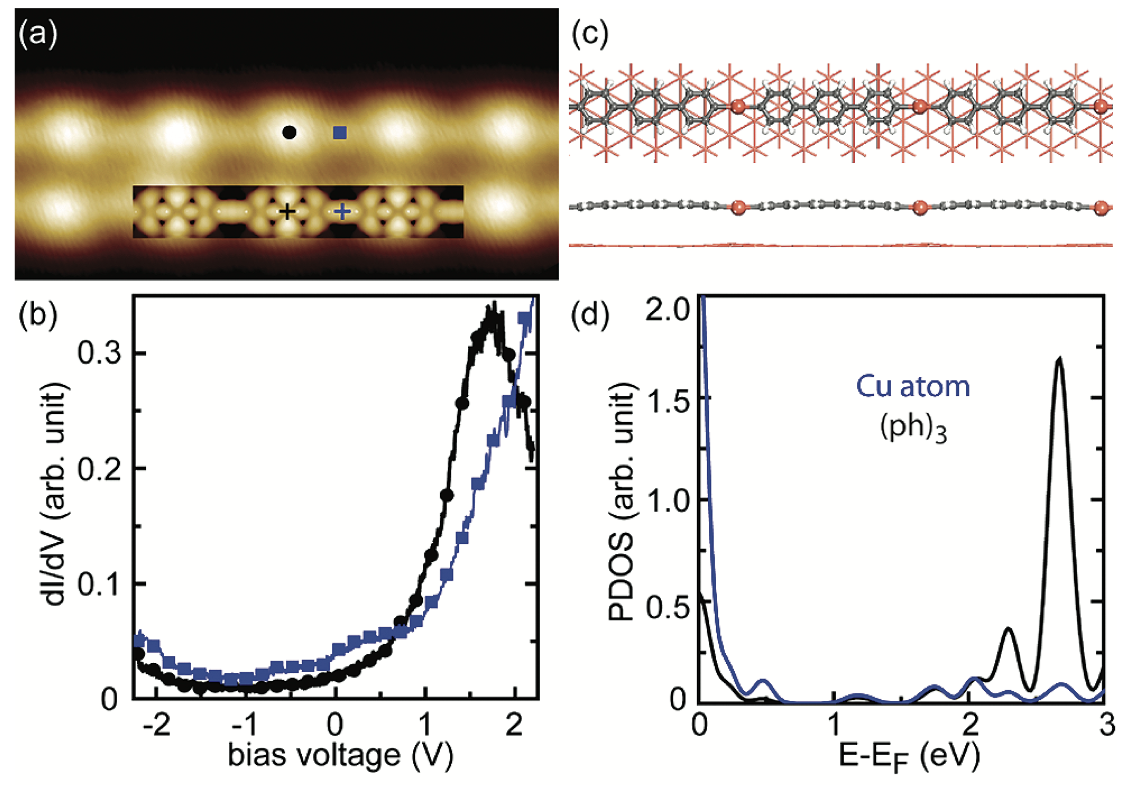
\includegraphics[scale=0.5]{achemso/Fig/Organometallic.png}
\caption{Carbon-Metal-Carbon Bridges in Organometallic Intermediate}
\label{fig:organ}
\end{figure}


\subsubsection{Formation of the C--C Bond}
Upon further annealing on the dimerized organometallic intermediates, the metal atoms are released, while two metalstable bonds are irreversibly converted into covalent bonds. In 2016, \citeauthor{jacs2016}\cite{jacs2016} reported the dimerization and trimerization of 1,4-dibromobenzene on Cu(100). It is found that organometallic intermediate is a relative stable phase in potential energy surface. A 0.7 eV of activation energy is required from the relatively stable organometallic intermediate to dimerized coupling product. And a 0.2 eV of activation is needed from dimerized coupling product the trimer. This result is consistent with the experimental data, which was investigated by neb\citeauthor{acsnano2013} in 2013. Same monomer dibromobenzene was deposited on Cu(100) surface, under STM image, organometalic intermediates are formed at RT, while the final coupling product need the temperature up to 500 K.

\begin{figure}[ht]
\centering
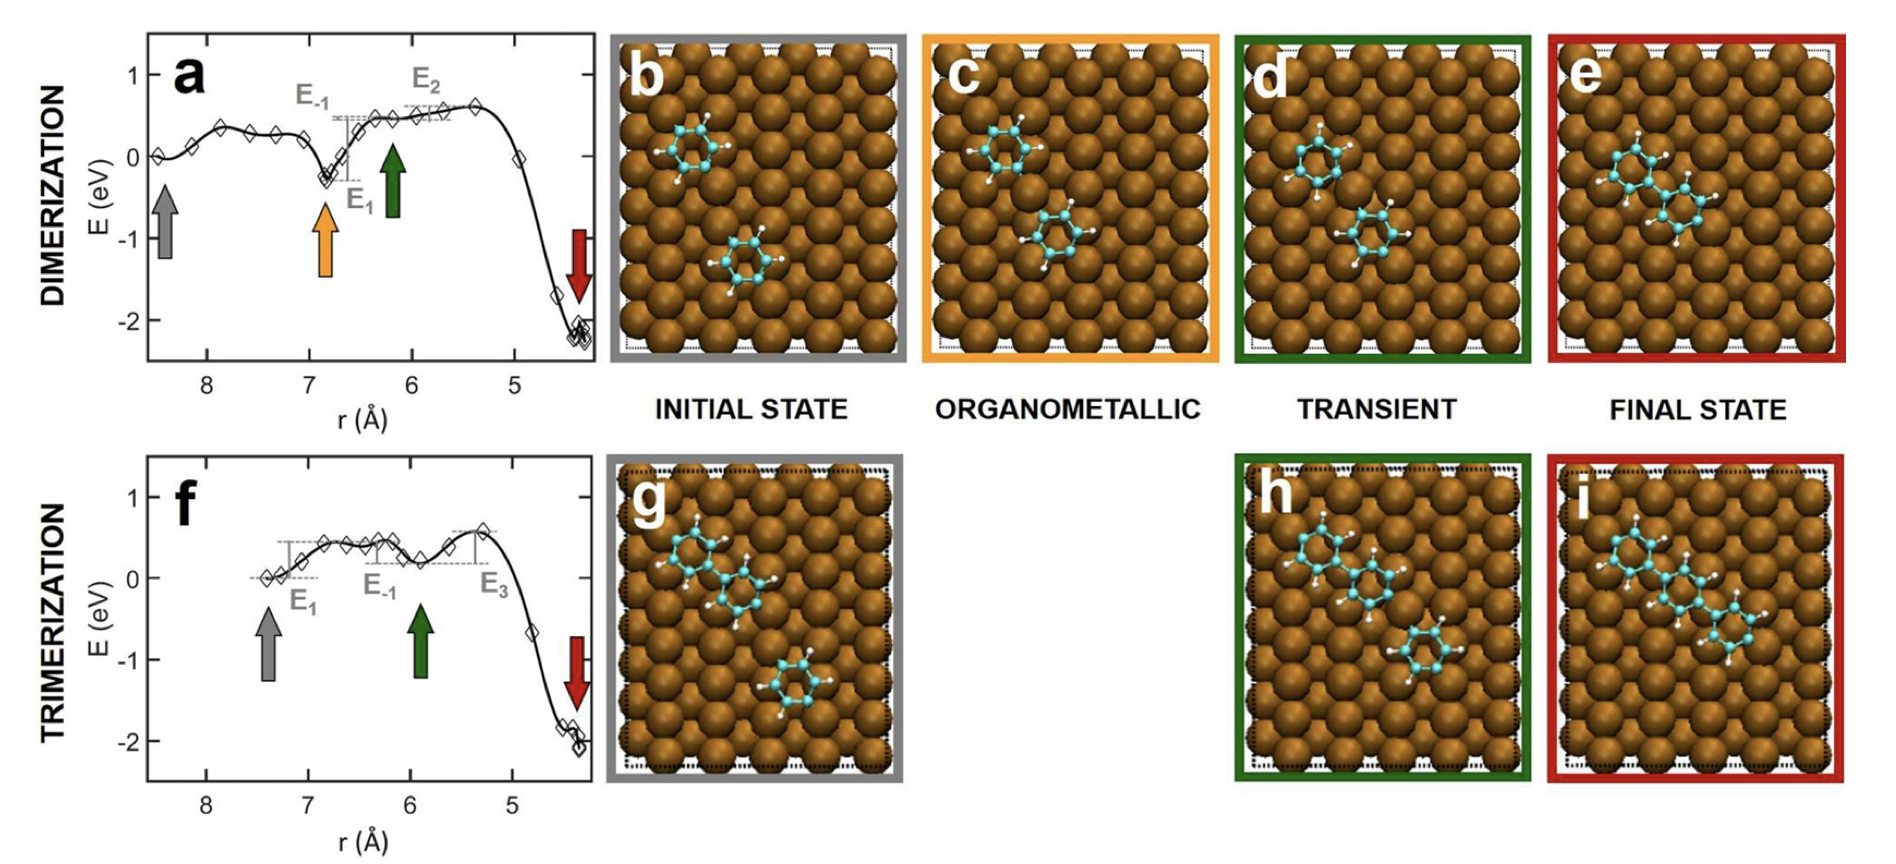
\includegraphics[scale=0.4]{achemso/Fig/Dimer_trimer.png}
\caption{Energy curve for dimerization and trimerizaiton coupling}
\label{fig:dimer}
\end{figure}


\subsection{Role of adatoms in the surface Ullmann coupling} 
Metal atoms are involved in the mechanism of Ullmann coupling containing five steps mentioned above. Investigation on the role of metal atoms in intermediates delivered a long-existence argument.
%%%%%%%%%%%%%%%%%%%%%%%%%%%%%%%%%%%%%%%%%%%%%%%%%%%%%%%%%%%%%%%%%%%%%%%%%%
%%The metal atoms may come from: (1) adatoms residing on metal surface; %%(2) metal atoms reside inside the metal surface. These two possibilities %%have been explored both experimentally and computationally in first %%three steps. \\
%%%%%%%%%%%%%%%%%%%%%%%%%%%%%%%%%%%%%%%%%%%%%%%%%%%%%%%%%%%%%%%%%%%%%%%%%%
Here the two terminology $Nature$ and $Origin$ will be used to distinguish the metal atoms in Ullmann coupling.
The nature of metal atoms: metal atoms can come from (1)surface atom or (2)adatoms.
The origin of adatoms: adatoms may come from (1)pre-exsiting adatom due to the the thermal fluctuations (At 298 K, the concentration of free adatoms and mono-vacancies $10^{-9}$ on Cu and Ag surfaces It increases to the order of $10^{-5}$ around 500 K). It increases to the order of 10 around 500K)[Figure.\ref{fig:2D-gas}] or (2)pulled out by the intermediates in Ullmann coupling. The nature of metal atoms and the origin of adatoms have been explored experimentally and computationally.

\begin{figure}[ht]
\centering
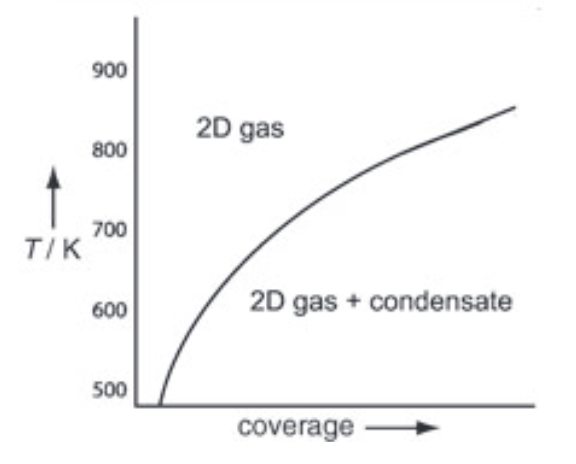
\includegraphics[scale=0.6]{achemso/Fig/2D-gas.png}
\caption{Adatoms Consentration on Metal at Elevated Temperature}
\label{fig:2D-gas}
\end{figure}


\subsubsection{Dehalogenation of Precursors}
Evidences already presented that metal adatoms are in assistance in the process of dehalogenation. In 2017, \citeauthor{chemeurope2017}\cite{chemeurope2017} explored the role of adatoms in the dehalogenation with iodobenzene on three different surfaces including Au(111), Ag(111) and Cu(111) based on DFT calculations.They compared the energetics of adatom formation on pristine metal surface and in the presence of iodobenzene. The comparison has shown that the energy of extracting a metal atom from the surface is decreased substantially from the 1.12-1.71~eV range to 0.13-0.24~eV range. Furthermore, the calculations have shown that the energy released in the process of adsorption of idobenzene and formation of metalorganic intermediates is sufficent to compensate the energy required for a metal atom extraction. [Figure.\ref{fig:3}]

\begin{figure}[ht]
\centering
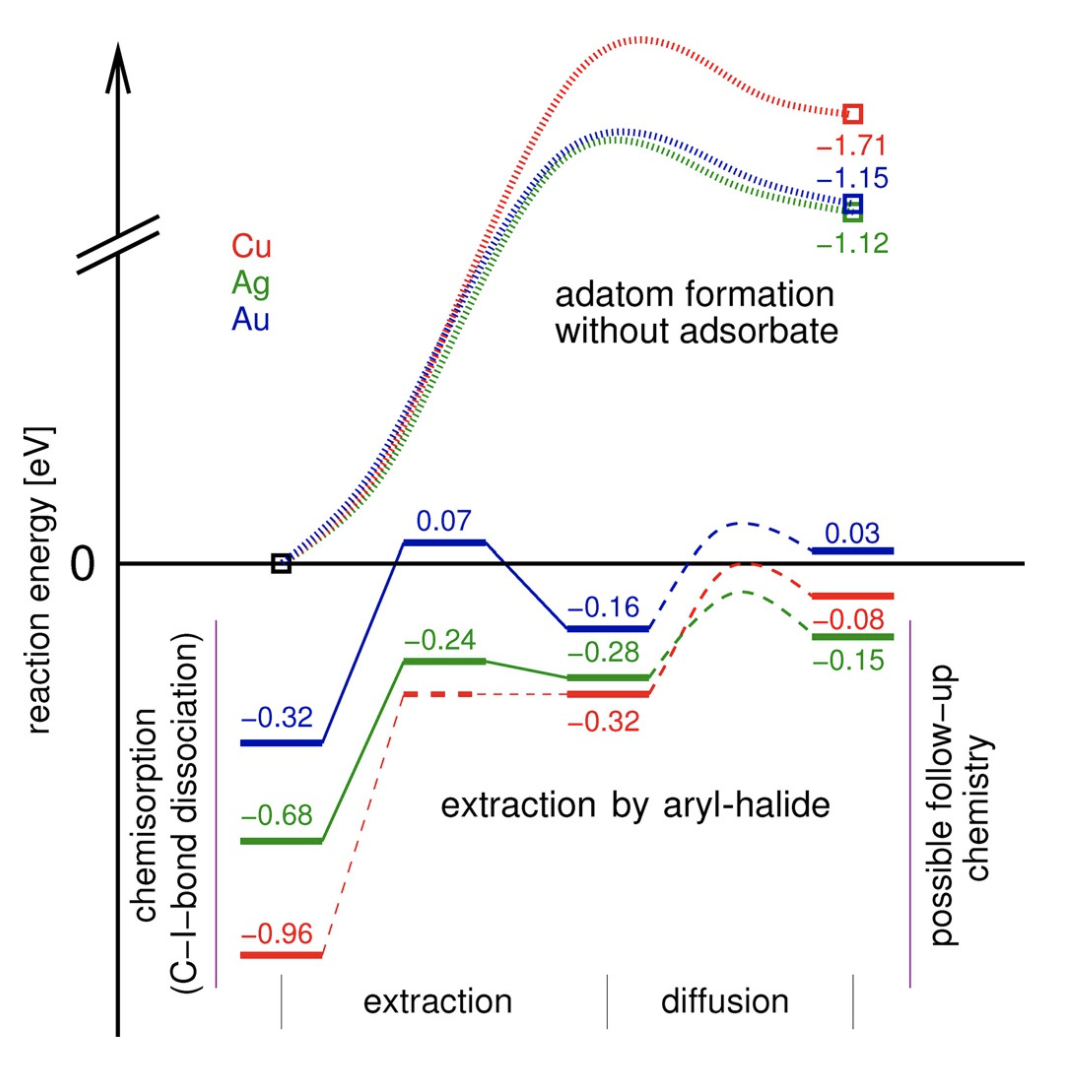
\includegraphics[scale=0.3]{Fig/Adatom-formation.png}
\caption{Energetics of adatoms formation}
\label{fig:3}
\end{figure}


\subsubsection{Diffusion of Two Dehalogenlated Radicals}
The diffusion process is involved in the interaction between single precursor radical and metal atom. 
In 2018, \citeauthor{jpcc2018}\cite{jpcc2018} investigated the mechanism of Ullmann coupling of 7,10-dibromofluoranthene (Br$_{2}$FL) on Au(111) via DFT calculations. Compared to simple phenyl rings that tend to form ~$36^\circ$ tilt angle with Cu(111) surface\cite{pccp2010}, the monoradical BrFL with only one Br atom removed stays almost parallel to Au(111) surface due to steric repulsion from the large backbone of BrFL radical and the substrate. And BrFL radical is found to lift surface Au atom out by 1.9 \si{\angstrom} from its initial position, which is much larger than 0.16 \si{\angstrom} produced by a phenyl ring. 

\citeauthor{acsnano2019}\cite{acsnano2019} also indicated 4-bromo-3$^{''}$-iodo-$p$-terphenyl radical interacts with the Cu atom inside the surface, and partially lift the Cu atom out from the surface while diffuses on Cu(111) surface. The conclusion 

\begin{figure}[ht]
\centering
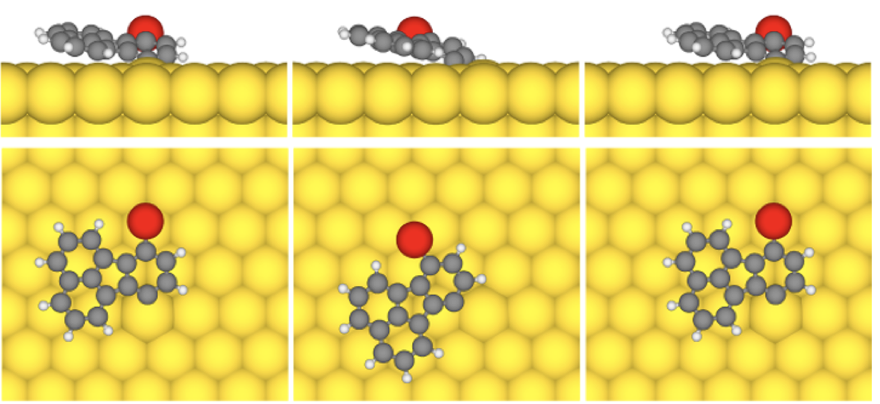
\includegraphics[scale=0.4]{achemso/Fig/Diffusion_path.png}
\caption{Diffusion}
\label{fig:diff}
\end{figure}


%%ZHZH: Dima changed a lot how to name the surface atom, adatom and lifted atom.
\subsubsection{The Formation of Organometallic Intermediates from Two Radicals}
The nature of the metal atom in dimerized organometallic intermediate has also been investigated through various approaches. In 2017, \citeauthor{acsnano2017}\cite{acsnano2017} analyzed structures of intermediates in the polymerization of bromotriphenylene to bistriphenylene on Cu(111) surface using STM/AFM and DFT calculations. Two computational models were considered: two triphenylene molecules bonded to an fully-out-of-surface adatom and two precursors bonded to an atom partially lifted from Cu surface [Figure.\ref{fig:5}]. It has been concluded that the structures observed in AFM are more consistent with computational adatom models. In particular, the C...C distance in organometallic intermediate is of 3.9 \si{\angstrom} measured by AFM, which is closer to the Cu adatom model (3.86 \si{\angstrom}) compared to the partially-lifted Cu atom model (3.42 \si{\angstrom}). Furthermore, the energy of formation of the adatom-containing intermediate from distant precursors is 1.74~eV lower than that of the intermediate with a partially lifted atoms. 


\begin{figure}[ht]
\centering
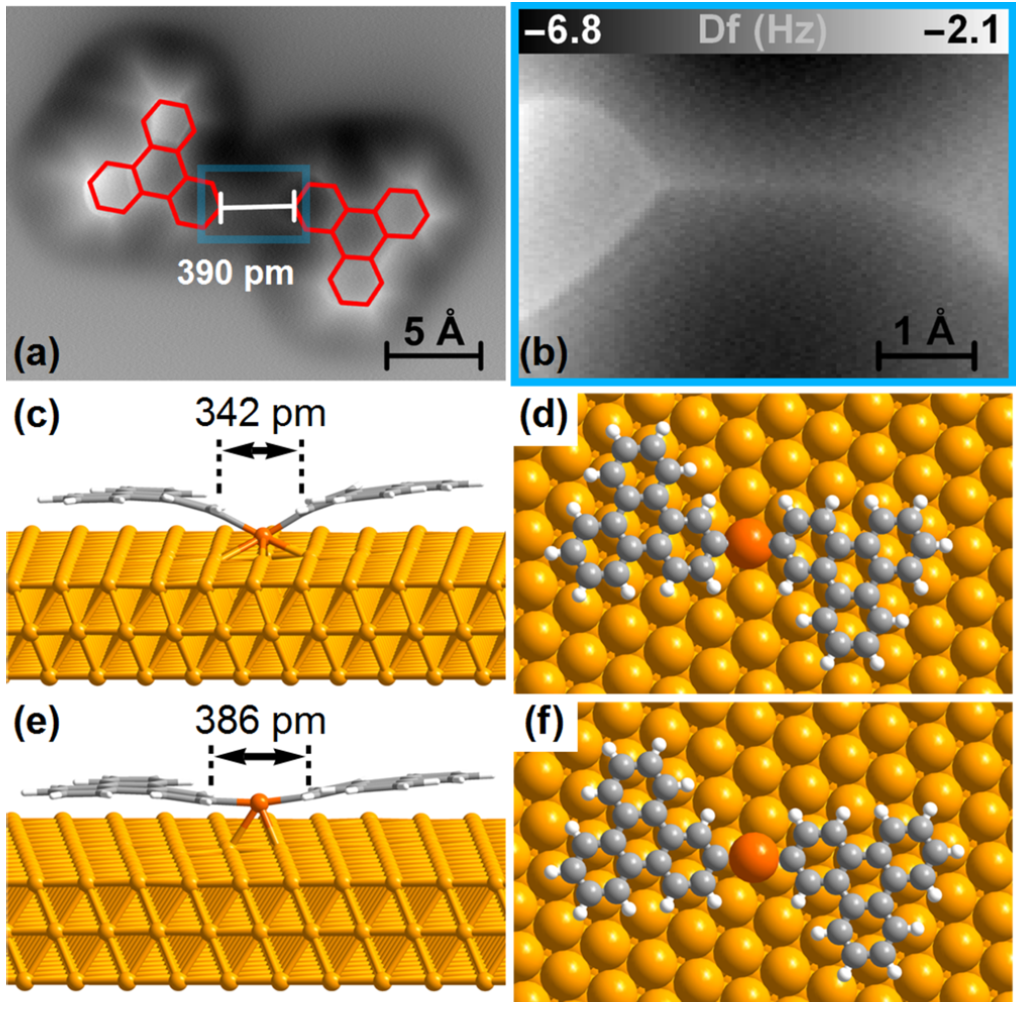
\includegraphics[scale=0.3]{achemso/Fig/distance.png}
\caption{distance}
\label{fig:5}
\end{figure}

%%ZHZH Dima suggests partial lifting should be discussed separately.

Then in 2019, not only the nature of metal atoms, but also the origin of the adatoms was discussed. The 2019 study of 4‐Bromo-3′′- iodo‐p‐terphenyl coupling on Cu(111), comparing experimentally and simulated AFM image, the Cu atoms in dimerized organometallic intermediate was again proven to be adatoms\cite{acsnano2019}. It was further suggested that these adatoms are generated by the extraction of two close single precursor radicals, instead of pre-exsiting adatoms from a statistic study of all intermediates species in the surface Ullmann coupling [Figure.\ref{fig:6}].
\begin{figure}[ht]
\centering
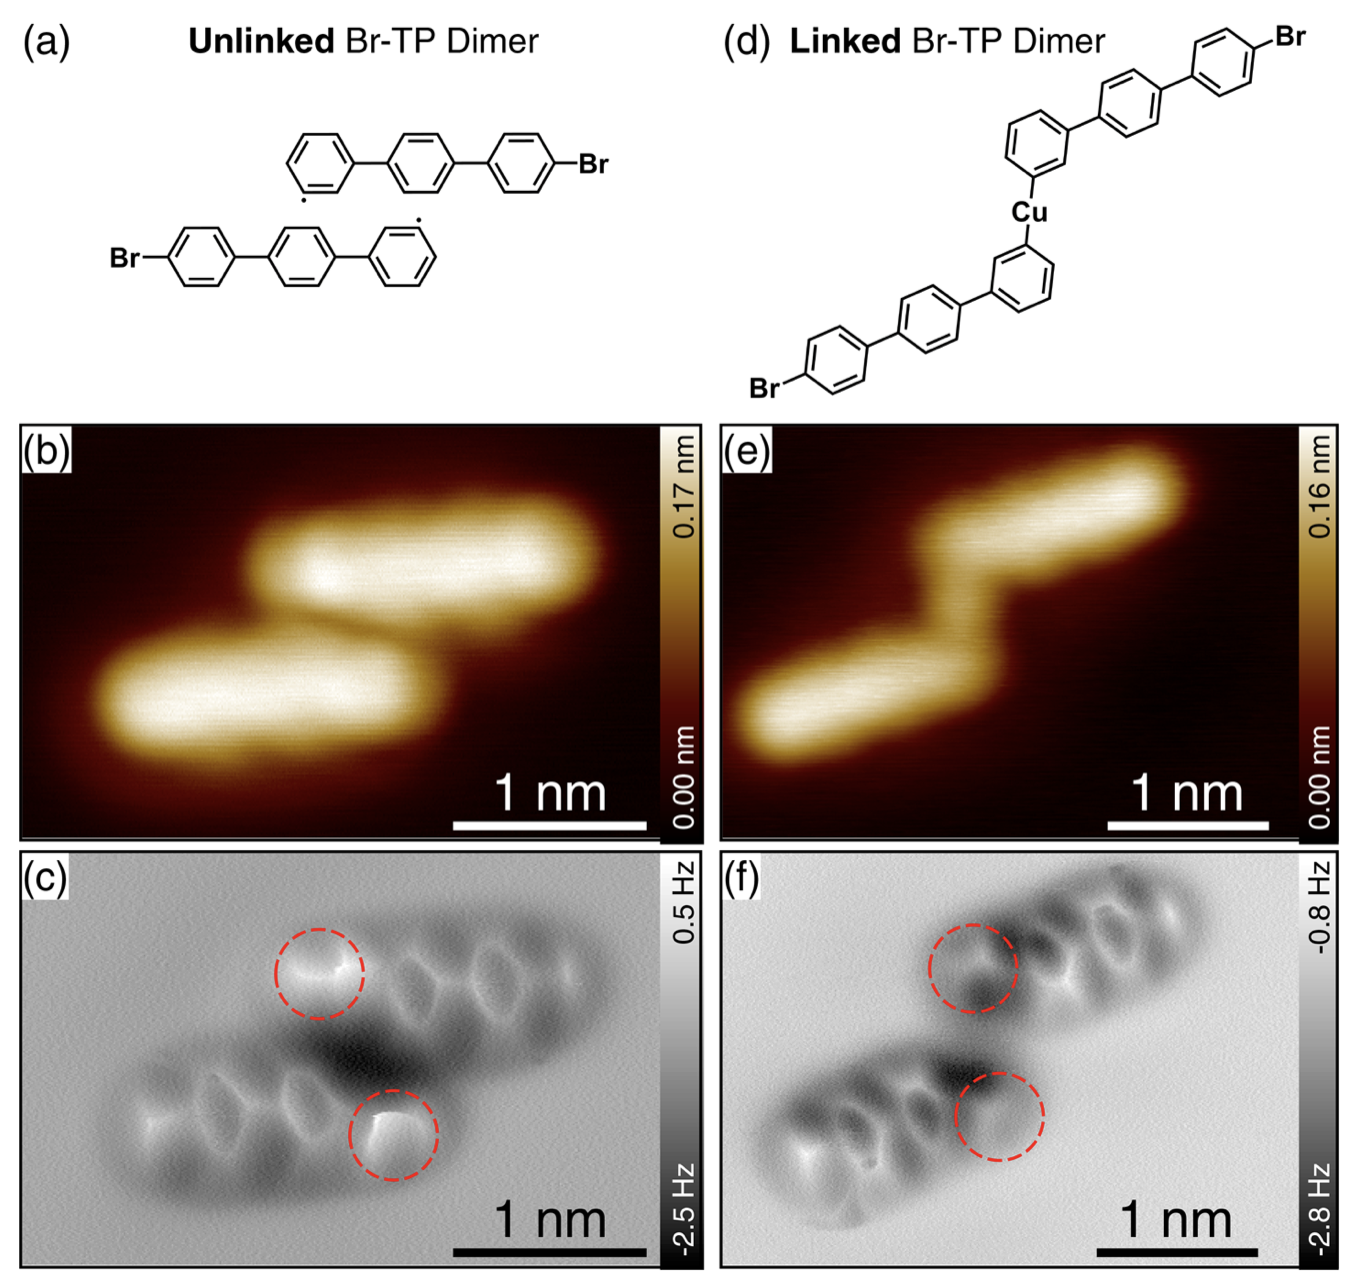
\includegraphics[scale=0.3]{achemso/Fig/AFM_prove.png}
\caption{AFM}
\label{fig:6}
\end{figure}

In addition, chlorinated prophyrin as precursor has been deposited on Cu(111)\cite{chematerial2019}. Based on DFT calculations, the Cu adatom mediated path is 3~eV lower than the direct dechlorination. And from STM image, some precursors are still intact at temperature 400~K, which should be already dehalogenated at lower temperature. It proves that the Cu adatoms are the limitaing agent [Figure.\ref{fig:prophyrin}].
\begin{figure}[ht]
\centering
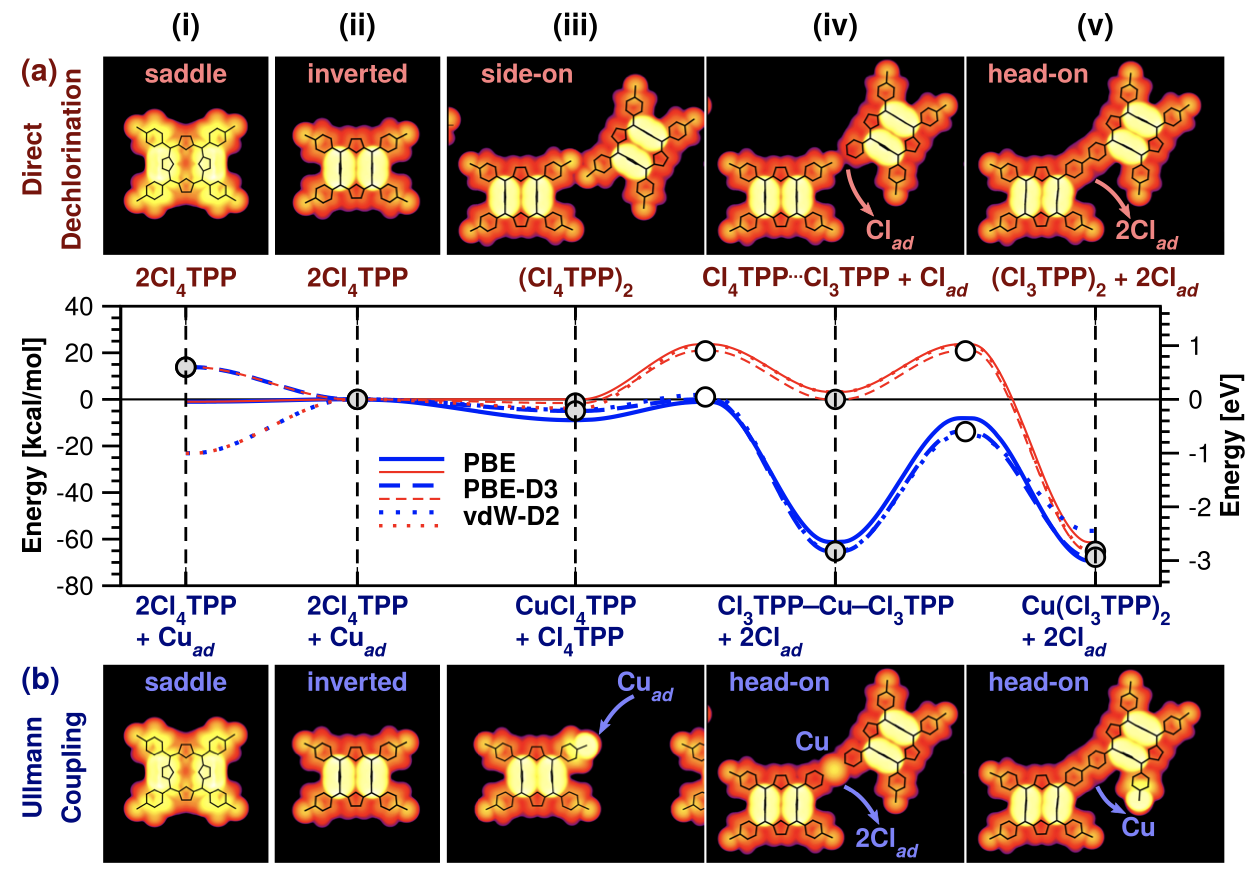
\includegraphics[scale=0.6]{achemso/Fig/Complete.png}
\caption{Prophyrin}
\label{fig:prophyrin}
\end{figure}

%%ZHZH Dima asked where is the analysis of formation of adatoms?



%%%%%%%%%%%%%%%%%%%%%%%%%%%%%%%%%%%%%%%%%%%%%%%%%%%%%%%%%%%%%%%%%%%%%
%% The appropriate \bibliography command should be placed here.
%% Notice that the class file automatically sets \bibliographystyle
%% and also names the section correctly.
%%%%%%%%%%%%%%%%%%%%%%%%%%%%%%%%%%%%%%%%%%%%%%%%%%%%%%%%%%%%%%%%%%%%%
\bibliographystyle{ieeetr}
\bibliography{achemso-demo}

\end{document}
